\subsection{Innan start}

Vid uppstart ritas knappar ut på displayen, se Figur \ref{fig:choose}. Med dessa knappar går
det att välja om en eller två banor ska vara aktiva och om de ska styras
autonomt av systemet eller manuellt med handkontroll. Det går också att ställa
in en referenstid mellan 12 och 15 sekunder med 0,5 sekunders intervall genom
att trycka på + och - på displayen. 
\begin{figure}
	\centering
	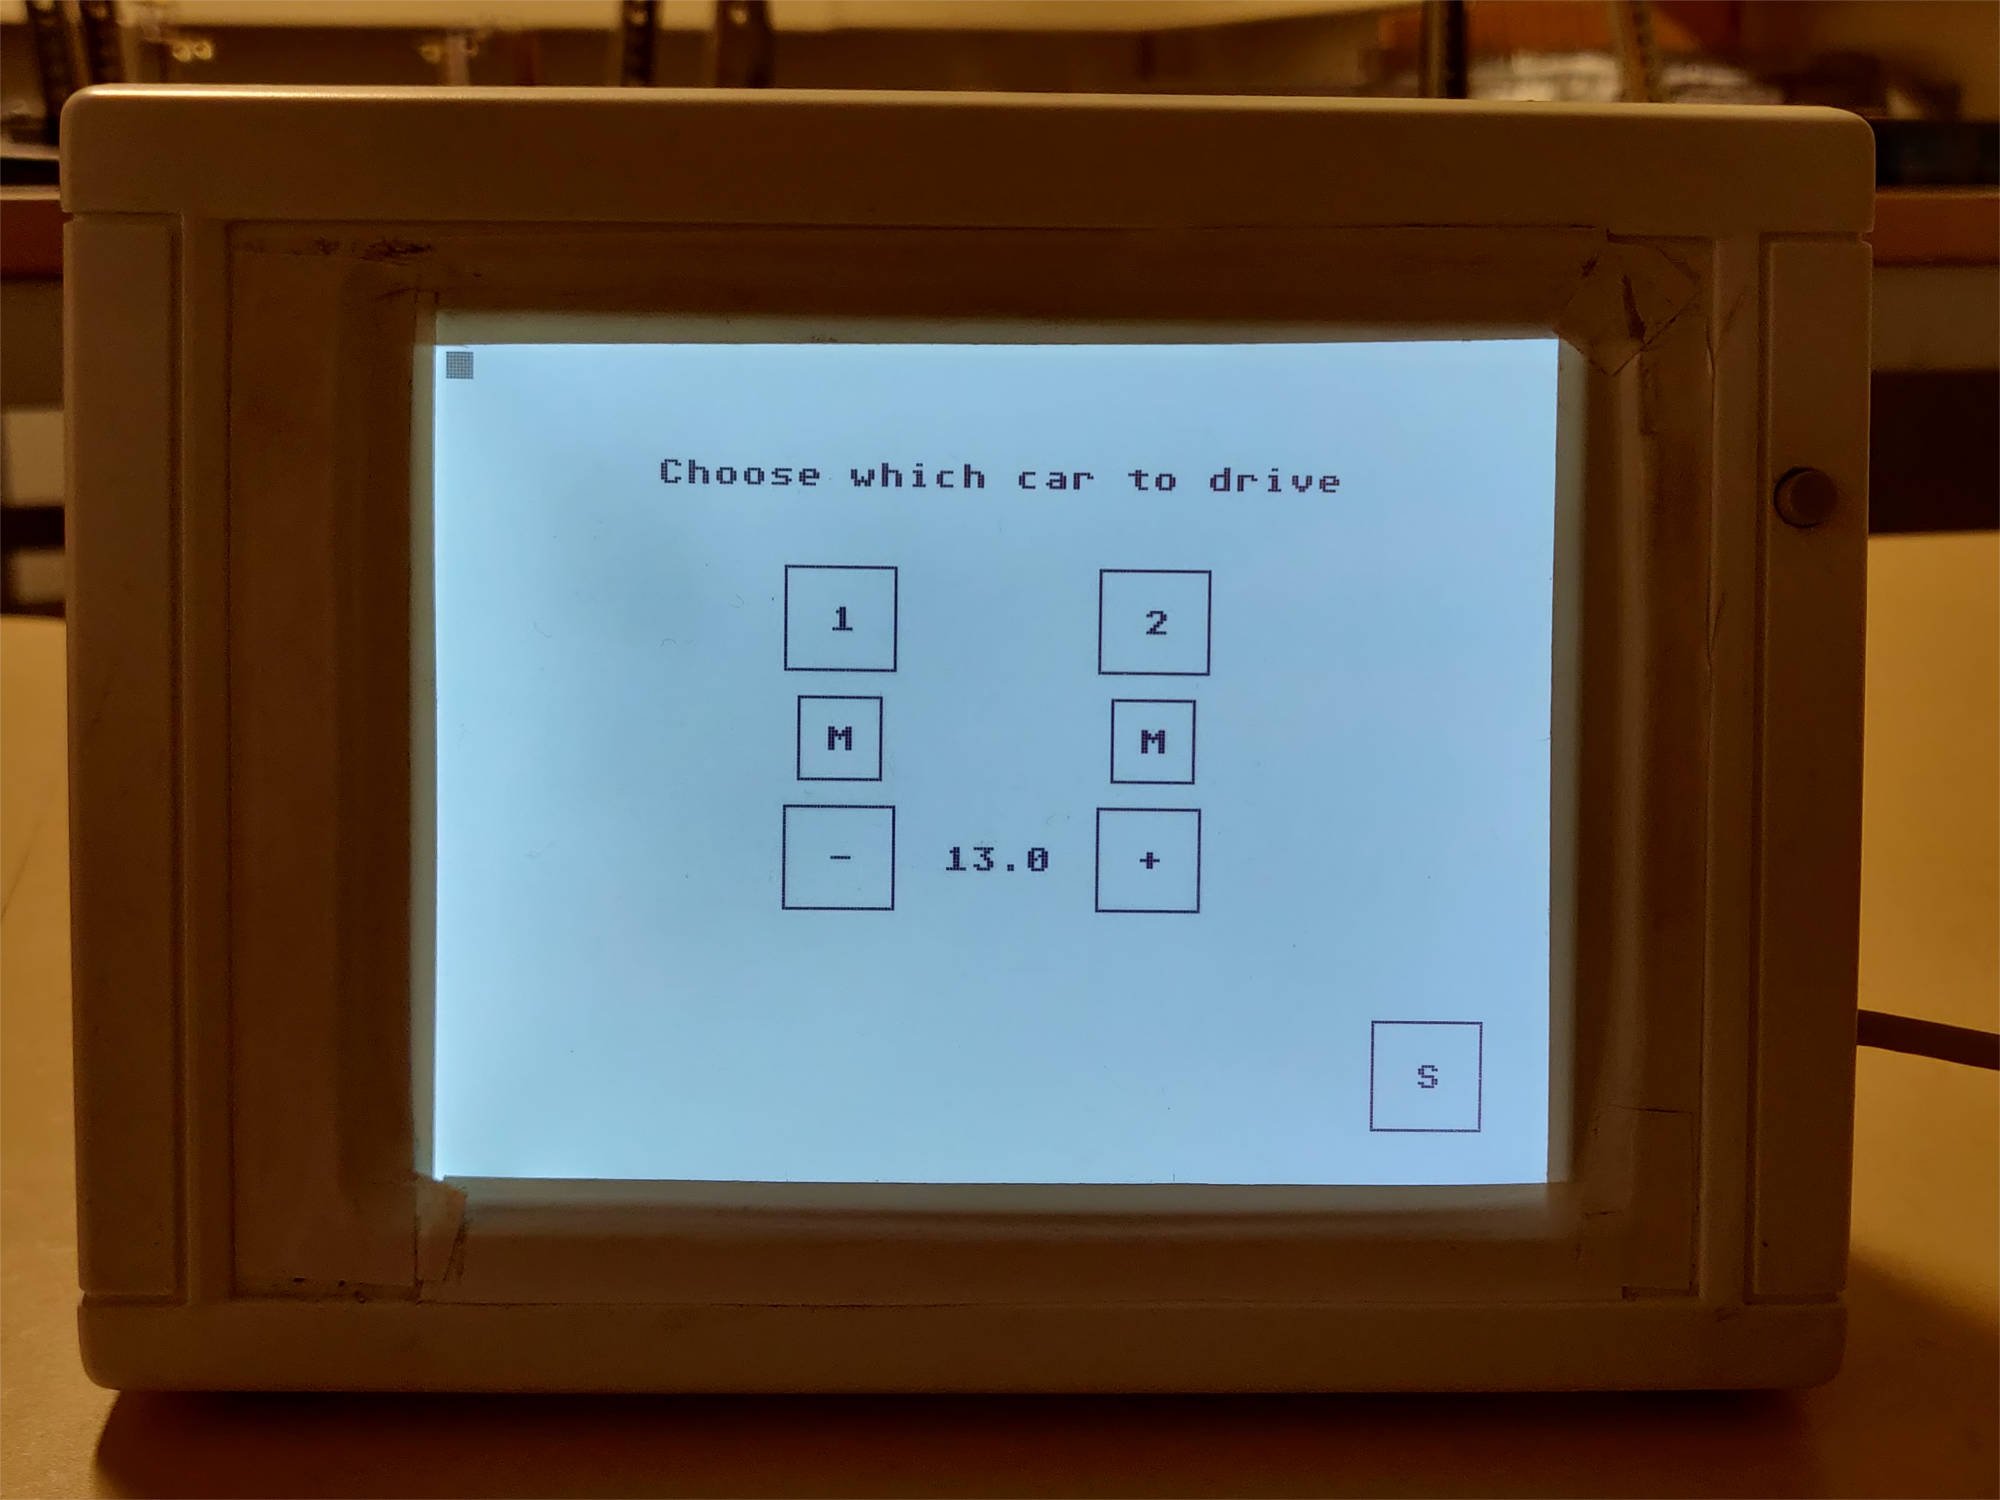
\includegraphics[width=0.75\linewidth] {Figures/choose1}
	%\caption{Display före start}
	%\label{fig:choose2}

	\vspace*{2\floatsep}% https://tex.stackexchange.com/q/26521/5764

	\centering
	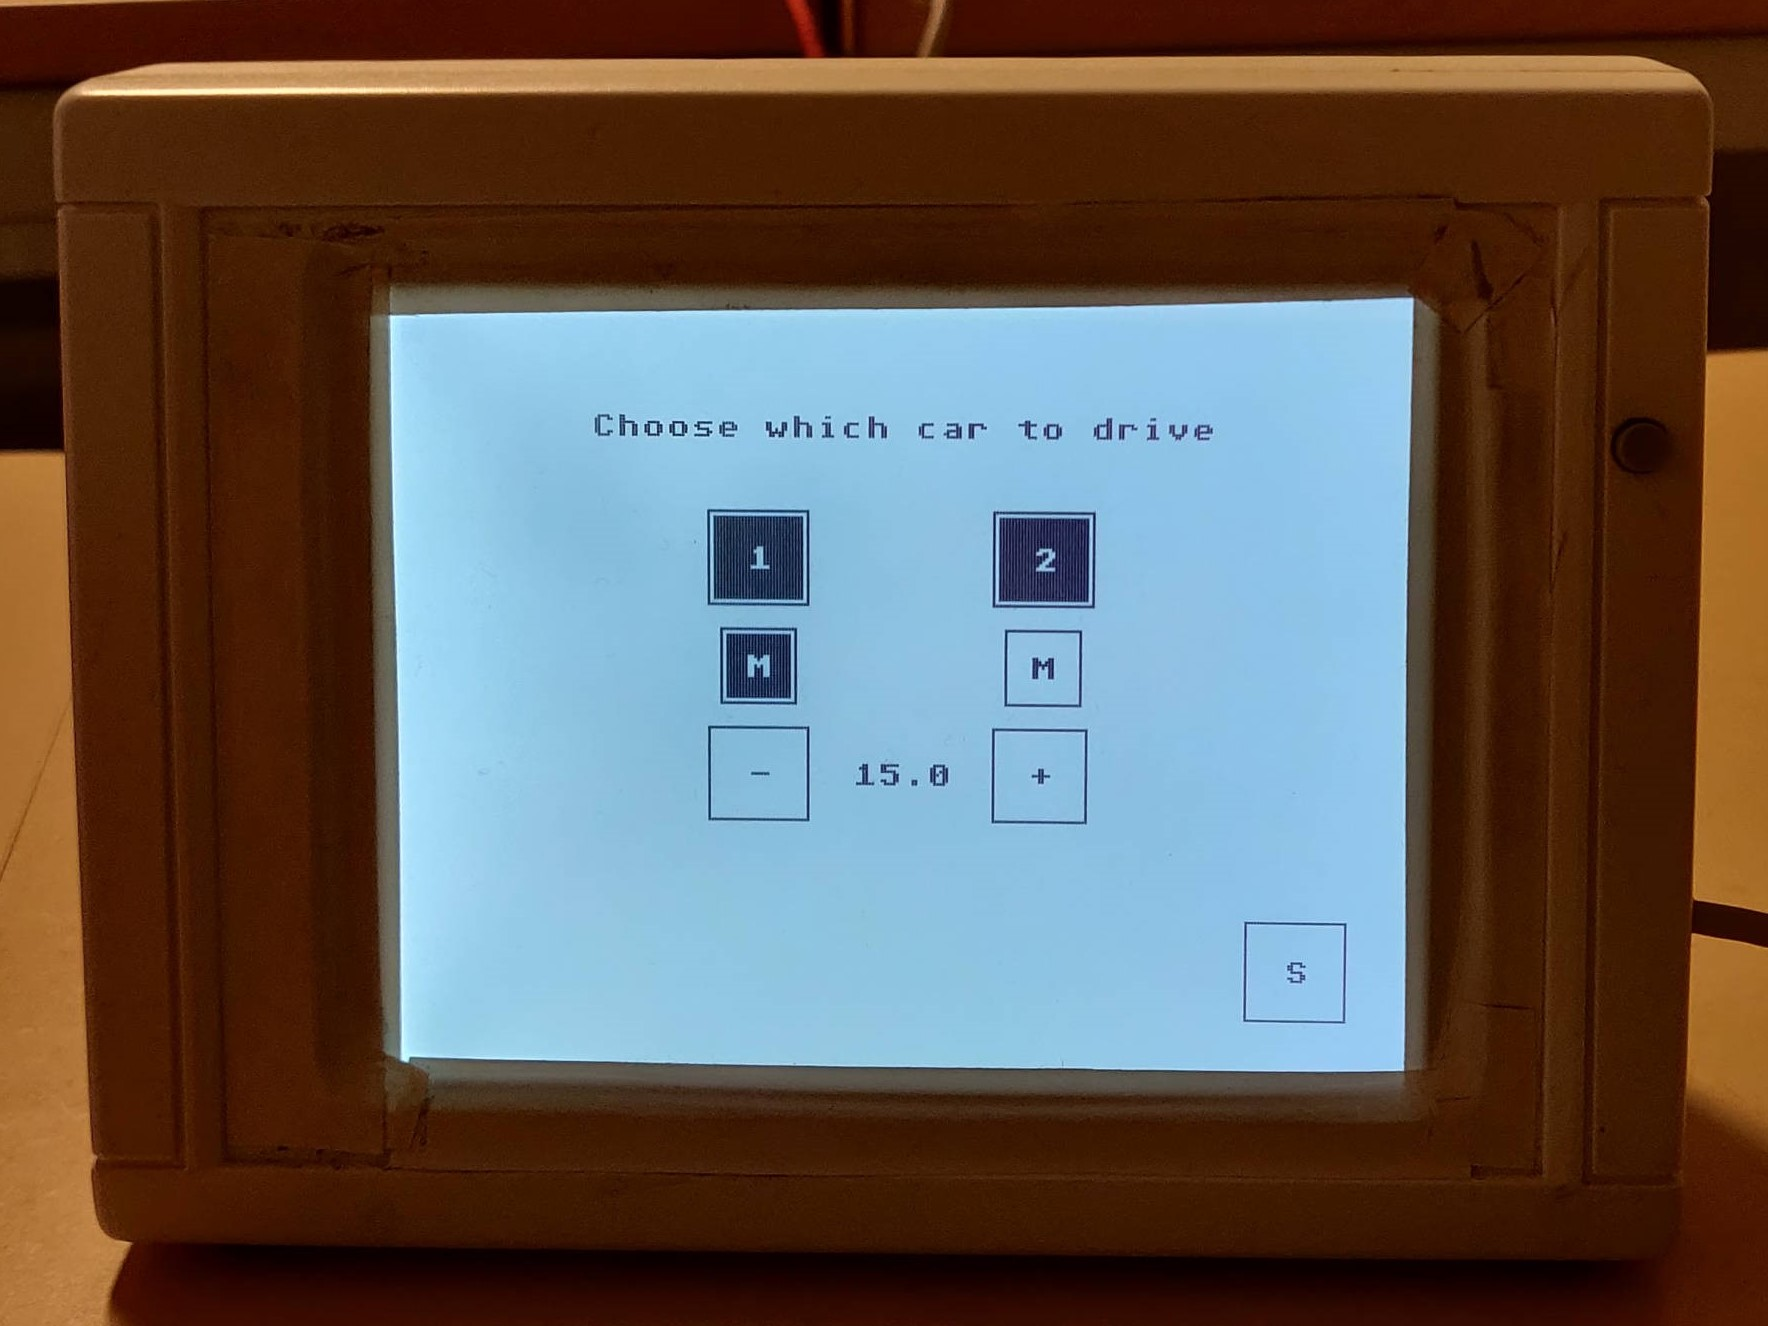
\includegraphics [width=0.75\linewidth] {Figures/choose2}
	\caption{Display före start.}
	\label{fig:choose}
\end{figure}
